\documentclass{article}

\usepackage{wrapfig}
\usepackage{graphicx}
\usepackage{amsfonts}
\usepackage{amsmath}

\begin{document}

\section{Problem 1}

I want to use linear programming to optimally plan
	time-investment into all of my classes.

\subsection{Decision Variables}
The decision variables for an optimal study plan are the
	number of hours per week spent studying for each
	class.
The number of hours per week will not vary each week.
On weeks with an exam instead of a problem set, the time
	will be used to study for an exam.
I have six classes, listed below.
I am a math major.
Some of the classes are math classes.

\paragraph{}
\begin{tabular}{|l|l|}
\hline
Class Name & Major? \\
\hline
QFT & no\\
\hline
Math Modeling & yes \\
\hline
Topology & yes \\
\hline
Combinatorics & yes \\
\hline
Robotic Manipulation & no \\
\hline
French & no \\
\hline
\end{tabular}

\paragraph{}
The decision variables are restricted by physical constraints.
For example, each one must be positive.
I'm assuming also that I do not have to spend an integer number of
	hours per week on each class.

There is also a constraint on the total number of hours spent per week.
It's more helpful to think about constraints per day:

\paragraph{}
\begin{tabular}{|l|l|}
\hline
Constraint & amount hrs / day \\
\hline
Sleep & 6 \\
\hline
Time with Spouse & 3 \\
\hline
Lecture & 3 \\
\hline
Transit Time & 1 \\
\hline
Meal Time & 1 \\
\hline 
\end{tabular}

\paragraph{}
This leaves 10 hours per day available to study.
On weekends, lecture is absorbed into spouse time.
Therefore, we conclude that there are 70 available total hours.

I am not placing any constraints on the total time spent on one class.

The decision space is therefore:

\[ D = \left\{ h \in \mathbb{R}^6 \mid \text{for } 1 \leq i \leq 6, h_i > 0; 
	\sum_{i=1}^6 h_i < 70 \right\} \]

\subsection{Optimization Goal}
I am trying to minimize the total time spent studying
	overall.
If $\vec{h} \in D$ is a set of decision variables, the total time per week
	is given by $\sum_{i=1}^6 h_i = \vec{h} \cdot \vec{1}$ ($\vec{1} = (1,1,1,1,1,1)$).
I am not trying to minimize time spent studying for one class over the other,
	I am treating each class equally.

\subsection{GPA Constraints}

I have two GPA constraints.
My GPA in all of my classes, the average of the grades in each class,
	must be above a 3.0.
My GPA in all of my major classes, again meaning the average, must be
	above a 3.5.

I need to determine how the number of hours spent on each class per week
	determines the grade in that class.
I'm going to assume that the number of hours spent per week is averaged out
	over the whole semester.

Since I want to use linear optimization, I am restricted to a linear relationship
	between the overall class grade and the number of hours spent studying
	for it.
I am going to try and determine two values for each class:
	the estimated grade (on a four point scale) that I will recieve if I do no work at all
		outside of lecture,
	and the estimated amount of hours per week to perfectly complete the problem set.
I am going to assume that the number of hours per week to complete the problem set
	perfectly is the same as the number of hours per week of studying required for
	the exam to get a perfect score.
This will simplify the analysis.

If a class has a no-effort grade $g_0$, and a requires $h_p$ hours of work per week for a
	perfect score, then the grade is given by the formula:

\[ g(h) = g_0 + (4 - g_0) \left( \frac{h}{h_p} \right) \]

This places an implicit constraint on the number of hours per week I can spend.
Since my grade in each class cannot be above 4.0 (if I have this kind of an attitude,
	I'm not going to get any A+'s), under the assumptions of my model I cannot
	spend more time in each class than the $h_p$ for that class.
We should revise the state space:

\[ D = \left\{ h \in \mathbb{R}^6 \mid \text{for } 1 \leq i \leq 6, 0 < h_i < {h_p}_i; 
	\sum_{i=1}^6 h_i < 70 \right\} \]




\subsubsection{Quantum Field Theory}

This class is a graduate class, so the grades will be higher.
However this class has regular reading assignments in addition to the problem set.
Each one of these reading assignments takes 2 hours, and there are two per week.
In addition, the homework is long and difficult, taking an average of eight hours.

The final is only 25 percent of the grade, in-class work is 10 percent, and the rest is homework.
This class is also very difficult for me, with new material.
I estimate that I will recieve a 1.0 with no work, and that I will need 12 hours
	of work per week to recieve a 4.0.

\subsubsection{Math Modeling}

This class is a 3000-level math class, so the grades will not be as 
	inflated as in graduate classes, but the grades will not be like
	those of weed-out classes.
This class has regular homework but gives significant weight to a project which
	I will count as "during lecture".
If I do alright on the tests, I think that I can get a 2.0 in the class with
	no work spent on the problem sets.
The problem set last week took about 4 hours, so being conservative, I estimate 
	that I can get a 4.0 in this class with 6 hours per week.

\subsubsection{Topology}

This class is a 4000-level math class, so grades will be relatively inflated.
In addition, the class time is spent doing the reading assignments.
The homeworks are weekly and relatively time consuming proof assignments.
Since there are tests and reading assignments that can be done in class,
	I estimate that I can recieve a 2.0 in this class with no work
	done outside of class.
I estimate that I can get a 4.0 in this class with 7 hours of work outside 
	of class per week.

\subsubsection{Combinatorics}

This class is a 4000-level math class, so I expect the grades to be relatively
	inflated.
The class time is spent on doing proofs, so if I only copy the statement of the
	proof at the end while using the class time to work on problem sets.
Through this technique, I think that I can achieve a grade of 1.5 in this class
	with no outside work, and complege a problem set in 5 hours.

\subsubsection{Robotic Manipulation}

This class is a 4000-level crosslisted CS/MechE class.
Most of the graded assignments are group projects, so I can get my group members
	to do most of the work through devious emailing and group member choice.
I therefore estimate that I can get a 2.5 without doing any of the work outside of class.
The work will take me 4 hours per week to get a 4.0, because I can start the 
	projects early.

\subsubsection{French}

French is a 2000-level class I'm taking for the language requirement.
The reading is discussed in class, so I don't have to do it if I make general
	comments responding to others.
The class has online homework assignments that need to be complete.
I speak french reasonable well, so I think that I can get a 2.5 in this class
	with no out-of-class work, and a 4.0 spending 1 hour per week.

\paragraph{}
I can summarize the parameters in a table:

\paragraph{}
\begin{tabular}{|l|l|}
\hline
$g_0$ (no-work grade) & $h_p$ (hours per week for 4.0) \\
\hline
1.0 & 12 \\
\hline
2.0 & 6 \\
\hline
2.0 & 7 \\
\hline
1.5 & 5 \\
\hline
2.5 & 4 \\
\hline
2.5 & 1 \\
\hline
\end{tabular}

\subsection{Summary of Constraints}

\subsubsection{Explicit Constraints}
\begin{enumerate}
\item I can't work more than the total number of available hours:
\[ h_1 + \dots + h_6 \leq 70 \]
\item The average grade must be above 3.0.
\[ \frac{\sum_{i = 1}^6 b_i + 4.0 \left( \frac{ h_i }{ \left( h_p \right)_i } \right)}{6} 
	\geq 3.0 \]
\item The average grade in major classes must be above 3.5
\[ \frac{\sum_{i = \{ 2,3,4 \}} b_i + 4.0 \left( \frac{ h_i }{ \left( h_p \right)_i } \right)}{3}
	\geq 3.5 \]
\end{enumerate}

\subsubsection{Implicit Constraints}
\begin{enumerate}
\item I can't work fewer than 0 hours per week.
For each $1 \leq i \leq 6$, $h_i \geq 0$.
\item I can get a maximum of 4.0 in each class,
so I cannot work longer than the number of hours required for a perfect.
For each $1 \leq i \leq 6$, $h_i \leq h_p$.
\end{enumerate}

\subsection{Results}

When I solve this linear constrained optimization problem with matlab,
	I find the following schedule:

\paragraph{}
\begin{tabular}{|l|l|}
\hline
Class & Hours per Week \\
\hline
QFT & 0.0 \\
\hline
Math Modeling & 1.5 \\
\hline
Topology & 0.0 \\
\hline
Combinatorics & 5.0 \\
\hline 
Robotic Manipulation & 0.0 \\
\hline
French & 0.375 \\
\hline
\end{tabular}

%%%%%%%%%%%%%%%%%%%%%%%%%%%%%%%%%%%%%%%%%%%%%%%%%%%%%%%%%%%%%%%%%%%%%%%%%%%%%%%%

\section{Problem 2: Robustness and Model Assumptions}

I want to find out how robust my predictions are.
Specifically, if the estimates of my parameters are flawed, how much
	can I expect this to change the results?
Will it make me study more than optimal?
How will it affect my GPA?

\subsection{Robustness Testing through Random Noise}

\begin{wrapfigure}{l}{0.35 \textwidth}
\begin{center}
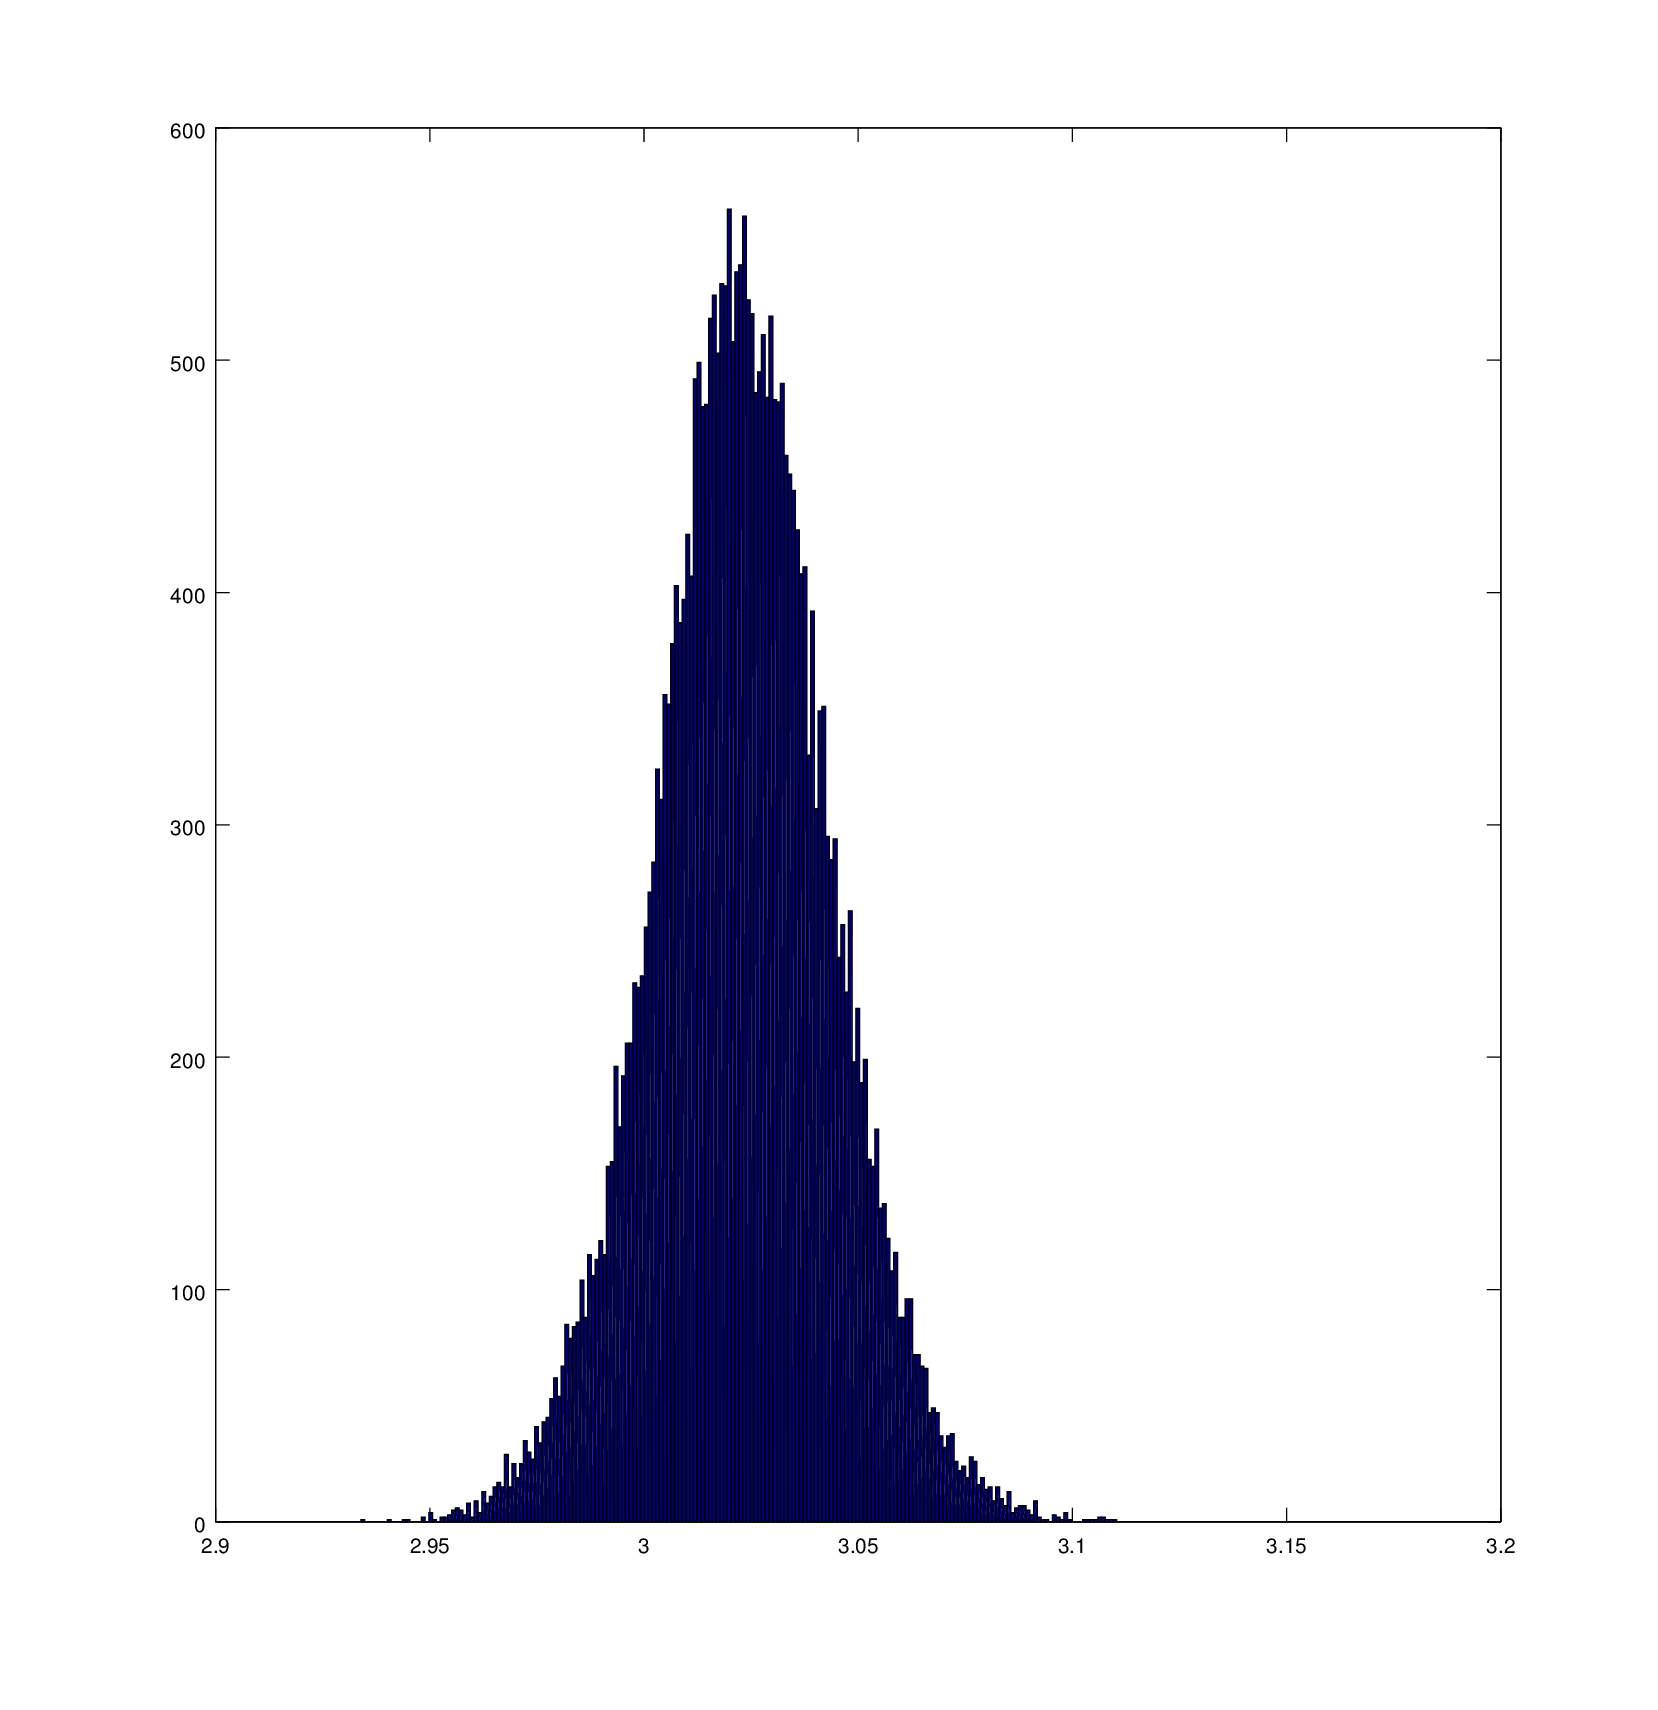
\includegraphics[width=0.3\textwidth]{stdiv-01-hist.png}
\end{center}
\caption{Total GPA's, gaussian noise added with $\sigma = 0.1$}
\end{wrapfigure}


I can do robustness testing through adding random noise to the 
	parameters, and evaulating how much it violates my 
	explicit constraints.
I will have to make sure that the implicit constraints are still satisfied.
Perturbations of the $b_i$ no-work grade parameter must leave the 
	parameter between $0.0$ and $4.0$.

Perturbations of the $h_p$ hours required for pset only need to remain positive.
We see that if we add gaussian noise to the parameters, the distribution of 
	possible gps's is approximately gaussian.
We can try and plot the ways that the mean and standard deviation of the GPA
	is related to the standard deviation of the added noise.

\begin{wrapfigure}{l}{0.5 \textwidth}
\begin{center}
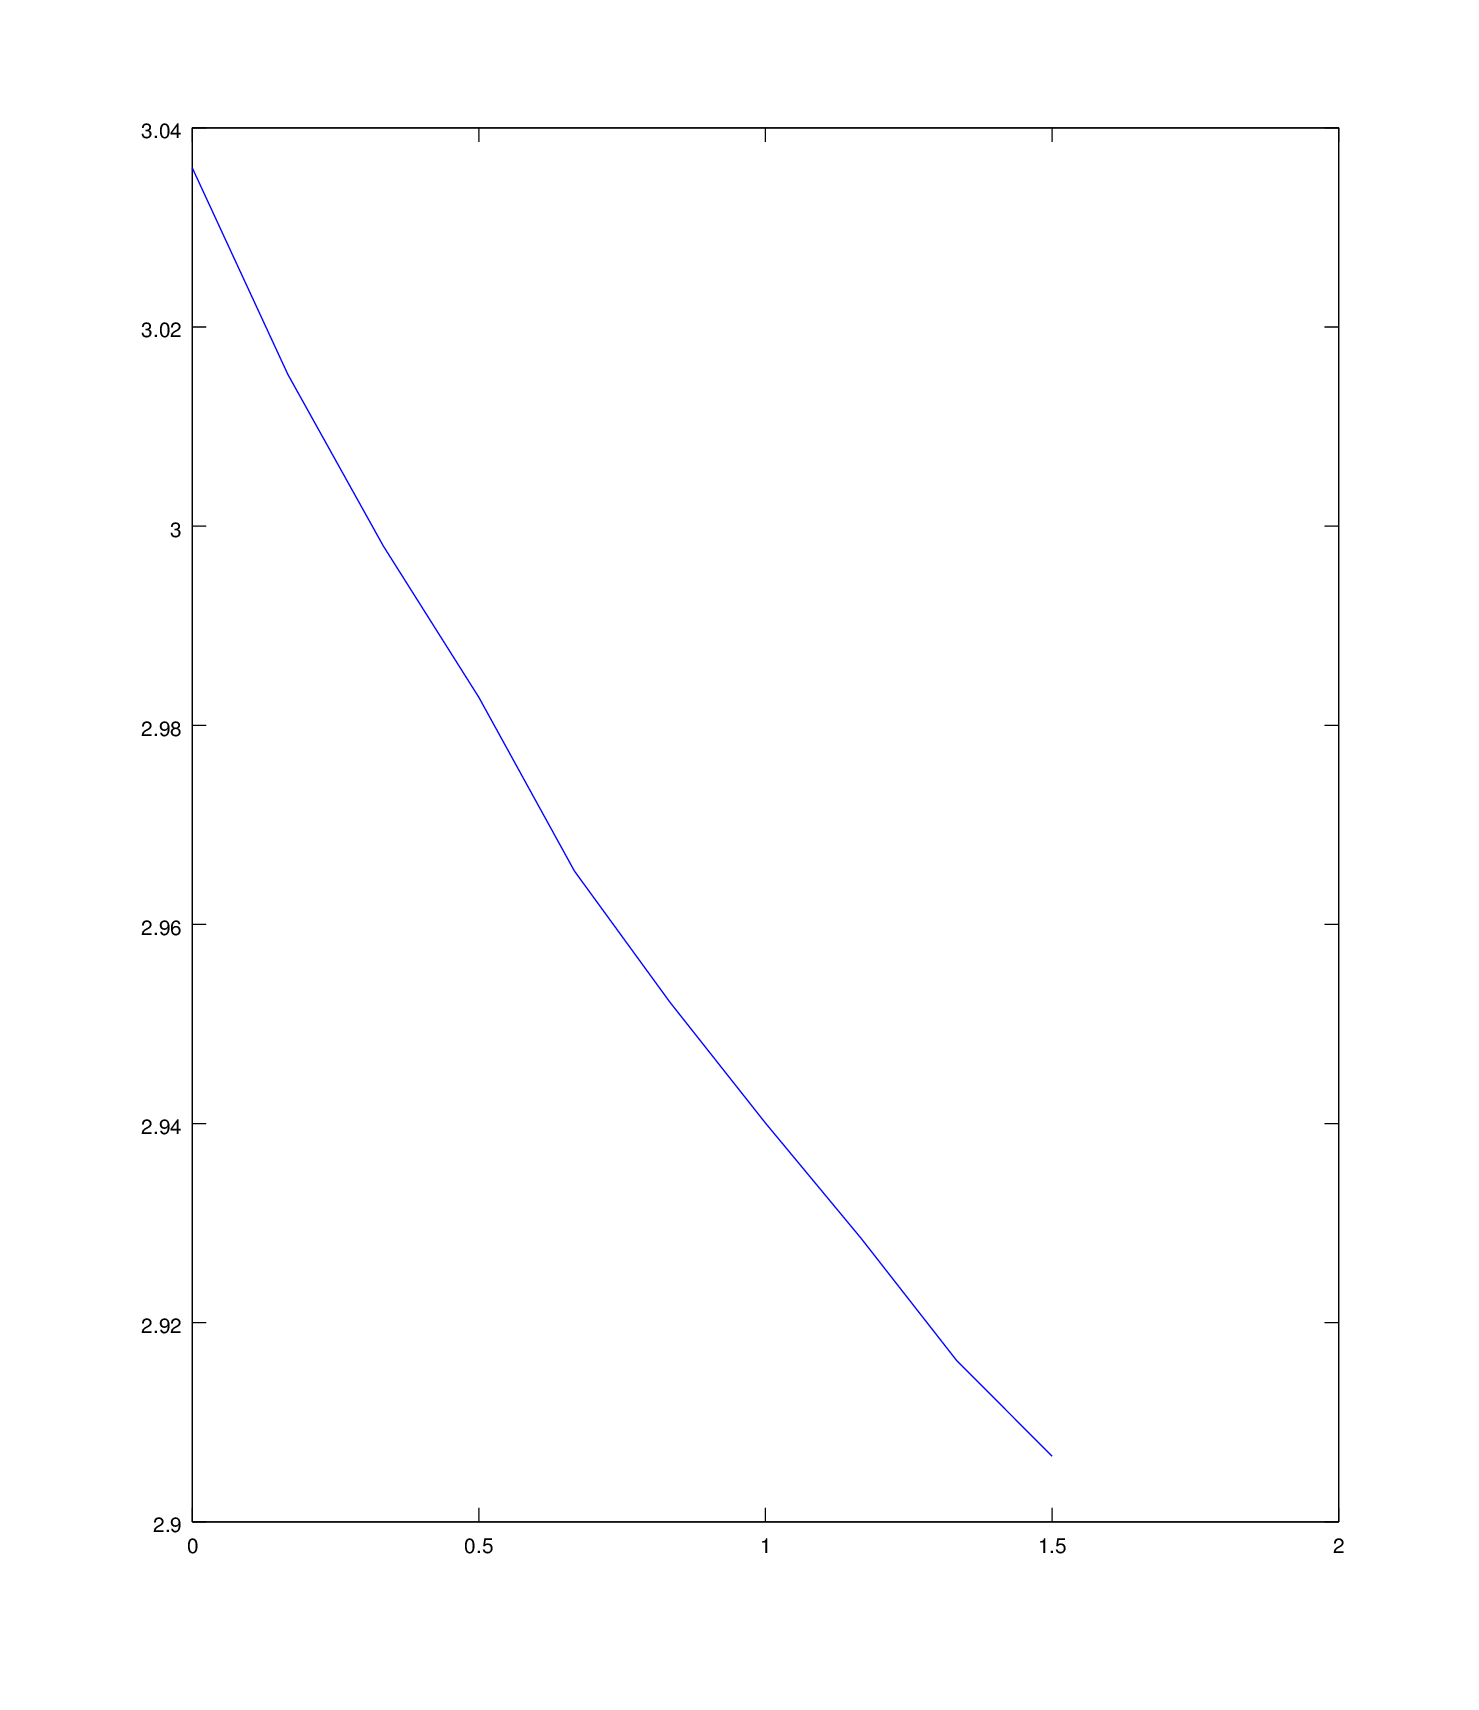
\includegraphics[width=0.45\textwidth]{means.png}
\end{center}
\caption{Mean Overall Grade, as $\sigma$ of noise on hours studying required is varied}
\end{wrapfigure}
\subsection{Other Neglected Aspects}

\begin{wrapfigure}{l}{0.5 \textwidth}
\begin{center}
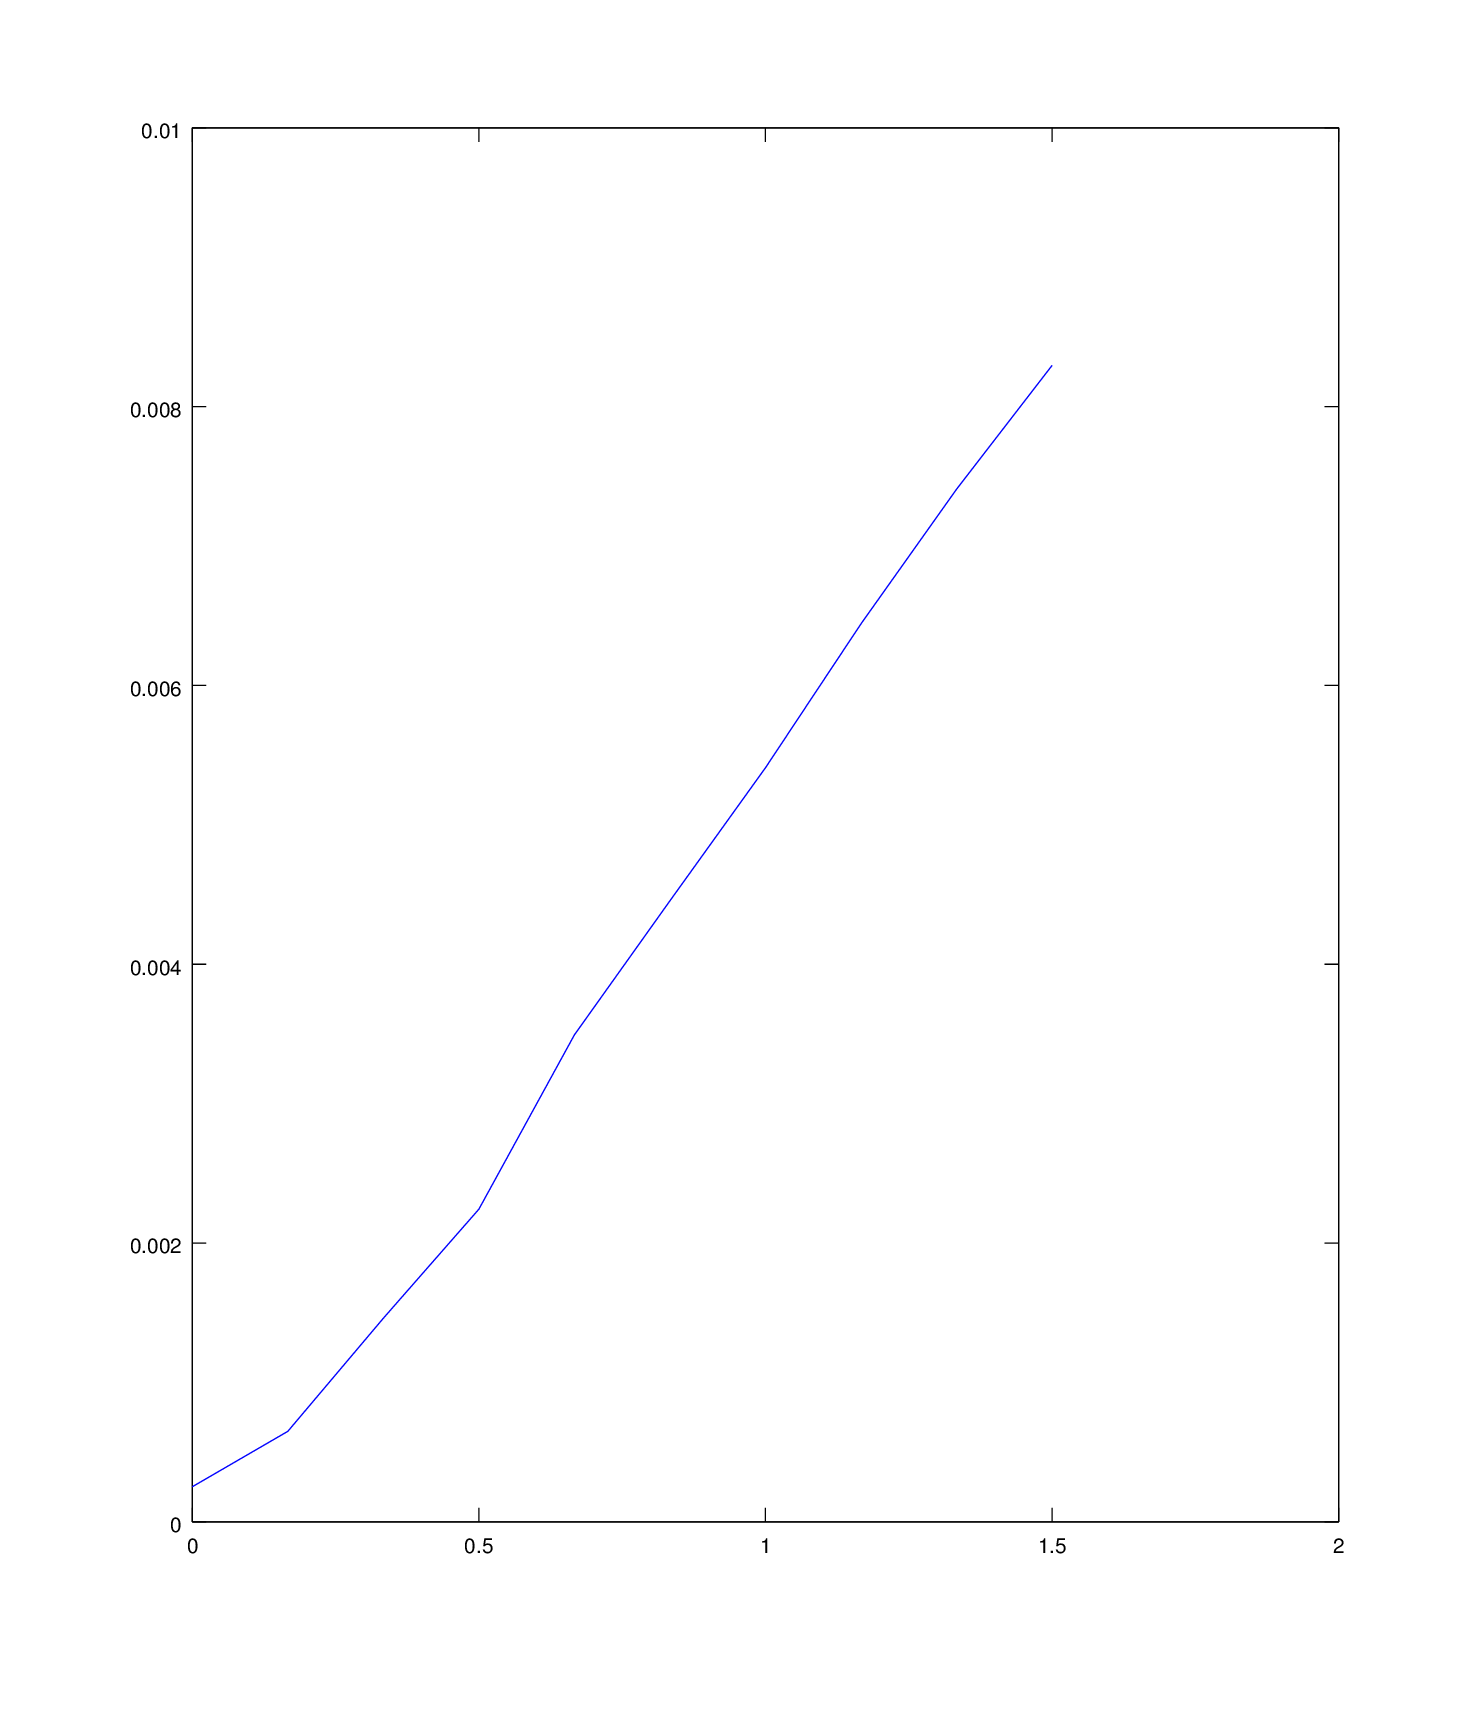
\includegraphics[width=0.45\textwidth]{standard-divs.png}
\end{center}
\caption{Standard Div of Overall Grade, as $\sigma$ of noise on hours studying required is varied}
\end{wrapfigure}
\subsection{Other Neglected Aspects}


Obviously, success in a class is determined by more than just the time
	spent studying for it.
It can be determined by how the study time is distributed over the week,
	and what types of studying is needed.
I haven't taken into account variances accross the semester in study time.
There could be additional parameters, representing studying vs. work on homework.
I could have several parameters for each class representing different study techniques.

Even if we restrict success in a class to be a function of only the time spent,
	there's very little reason to expect the relationship to be linear.
Studying also has significant nonlinear effects.
A 1-minute studying session is almost certainly not 1/100th of a 100 minute 
	study session.
I don't know whether it's more effective or less effective.
I definitely expect that the function $g(h)$ will saturate on the high end.

The linear objective function is pretty accurate.
It could be generalized by weighting different classes differently,
	to express a preference in studying for one class over another. 
For example, suppose I strongly dislike french, 5x more than I dislike studying
	for other classes.
Instead of optimizing to minimize $(1,1,1,1,1,1) \cdot \vec{h}$, I can try to minimize
	$(1,1,1,1,1,5) \cdot \vec{h}$.
The results are summarized below.

\paragraph{}
\begin{tabular}{|l|l|l|}
\hline
Class & Hours per Week (Original) & Hours per Week (new)\\
\hline
QFT & 0.0 & 0.0\\
\hline
Math Modeling & 6.0 & 6.0\\
\hline
Topology & 1.75 & 1.75\\
\hline
Combinatorics & 5.0 & 5.0\\
\hline 
Robotic Manipulation & 0.0 & 4.0\\
\hline
French & 0.375 & 0 \\
\hline
\end{tabular}


\section{Problem 3}

\subsection{``Spread'' and ``Relative Spread''}

The ``spread'' is the difference between the maximum final value,
	and the minimum final value.
The ``relative spread'' attempts to normalize this value, by dividing
	by the expected value of the population in the continuum limit.
So, the relative spread compares the difference in highest and lowest values
	to the expected value of the population.
This is good at making sure that differences in the spread which are extremely
	small compared to the actual values of the population can be distinguished
	from differences in spread which correspond to a significiant portion
	of the population.

Since the spread and relative spread use the maximum and minimum values exclusively,
	I expect that running more samples would get more and more unlikely behavior,
	represented as strings of good or bad luck reproducing.
Therefore the spread and relative spread should increase when more trials are run.

For example, on the lecture script, I get a relative spread of 0.646
	when I run with 80 random sequences,
	and 0.531
	when I run with 40.

The spread is good for determining deterministic and stochastic models of growth
	because it represents how much of a deviation from the expected value
	we might expect when trying to make decisions based on the model.

\subsection{Different Initial Population Sizes}

How does varying the initial population size affect the relative spread?

\paragraph{}
\begin{tabular}{|l|l|}
\hline
initial population & relative spread after 20 iterations\\
\hline
2 & 1.3065 \\
\hline
3 & 0.9528 \\
\hline
4 & 0.7884 \\
\hline
5 & 0.9000 \\
\hline
10 & 06211 \\
\hline
20 & 0.4424 \\
\hline
40 & 0.2984 \\
\hline
80 & 0.1793 \\
\hline
160 & 0.1050 \\
\hline
\end{tabular}

\paragraph{}
The relative spread is a good way of determining how well the deterministic
	model reflects the stochastic model.
The lower the relative spread, the more accurate I can expect the deterministic model
	to be.

\subsection{Different Iteration Times}

How does adding more iterations affect the relative spread?

\paragraph{}
\begin{tabular}{|l|l|}
\hline
number of iterations & relative spread \\
\hline
20 & 0.65233 \\
\hline
25 & 0.58804 \\
\hline
30 & 0.60614 \\
\hline
\end{tabular}

It seems like adding more iterations decreases the relative spread,
	which seems like a restatement of the so-called ``law of large numbers'', 
	that the larger these sequences get, the less ``remarkable'' they 
	become.

\end{document}
